\documentclass[13pt,a4paper]{article}

\usepackage[utf8]{inputenc}
\usepackage[T1]{fontenc}
\usepackage[english]{babel}
\usepackage{amsmath}
\usepackage{amsfonts}
\usepackage{amssymb}
\usepackage{hyperref}
\hypersetup{pdfstartview = {XYZ null null 1.00}}
\usepackage[hmargin=2cm,vmargin=3cm]{geometry}
\usepackage{wrapfig}
\usepackage{enumitem}
\usepackage{fancyhdr}
\usepackage{float}
\usepackage{eurosym}
\pagestyle{fancy}
\usepackage{setspace}

\usepackage{titlesec}
\usepackage{pgfplots}
\usepackage{pgfplotstable}

\newcommand{\hsp}{\hspace{20pt}}
\newcommand{\HRule}{\rule{\linewidth}{0.5mm}}
\usepackage[utf8]{inputenc}
\usepackage[francais]{babel}
\usepackage[left=1cm,right=1cm,top=2cm,bottom=2cm]{geometry}
\usepackage{amsmath}
\usepackage{amsfonts}
\usepackage{amssymb}
\usepackage{setspace}
\usepackage{graphicx}
\usepackage{color}
\definecolor{freemokmassoft}{rgb}{0,0,1}
\usepackage{fancybox}
\usepackage{fancyhdr}
\usepackage[dvipsnames]{xcolor}
\usepackage{wrapfig}
\usepackage[T1]{fontenc}
\usepackage{tikz}
\usetikzlibrary{positioning}
\usetikzlibrary{shapes, arrows, positioning, mindmap, backgrounds}

\begin{document}

\titleformat{\paragraph}
{\normalfont\normalsize\bfseries}{\theparagraph}{1em}{}
\titlespacing*{\paragraph}
{0pt}{3.25ex plus 1ex minus .2ex}{1.5ex plus .2ex}

\fancyhead[R]{\bf Promotion : 2023/2024\\
                  Amine OUGUENOUNE}
\fancyhead[L]{\bf Sorbonne Université : Sciences \\ Master AR : Ingénierie  \\ des systèmes intelligents \\  
1\up{ère} année \\ UE : Missions en entreprise \\}

\fancyhead[C]{
\includegraphics[scale=0.2]{logo.jpg}}

\fancyfoot[R]{}
\fancyfoot[L]{}
\fancyfoot[C]{\bf \thepage}
\pagestyle{fancy}

\vspace*{5cm}

  \begin{sffamily}
  \begin{center}
    \vspace{1cm}
   
    \HRule \\[0.4cm]
    { \huge \bfseries \bf \huge Rapport d'alternance :\\
    Data science et software engineering dans le secteur bancaire \\ 
    \normalsize \bf Référent d'entreprise: Emmanuel Chauvin, BNP Paribas ITG \\
    \bf Référent académique : Henri Boutin, IRCAM / Sorbonne université \\
 [0.4cm] }

    \HRule \\[2cm]
    
\includegraphics[scale=0.2]{logo_bnp.png}
    \\[1cm]
    \vfill
  \end{center}
  \end{sffamily}
%%%%%%%%%%%%%%%%%%%%%%%%%%%%%%%%%%%%%%%%%%%%%%%%%%%%%%%%%%%%%%%%%
\newpage


\fancyhead[]{}
% Créer le glossaire

\tableofcontents 
\vspace{5cm}






\newpage
\section*{Glossaire}
\thispagestyle{empty}

\begin{description}
    \item[API] Application Programming Interface.
    \item[BAAI] Beijing Academy of Artificial Intelligence.
    \item[BERT] Bidirectional Encoder Representations from Transformers, a pre-trained NLP model.
    \item[BP2S] BNP Paribas Securities Services, providing asset servicing and administration solutions.
    \item[CIB] Corporate and Institutional Banking, focusing on corporate finance and global banking solutions.
    \item[CI/CD] Continuous Integration/Continuous Deployment, a set of practices in software engineering.
    \item[CSRD] Corporate Sustainability Reporting Directive, a regulation for corporate reporting on sustainability.
    \item[DFS] Depositary and Fiduciary Solutions, managing custodial and fiduciary duties.
    \item[ESG] Environmental, Social, and Governance, criteria for sustainable and ethical investments.
    \item[FAISS] Facebook AI Similarity Search, a library for efficient similarity search and clustering.
    \item[Fine-Tuning] The process of adjusting a pre-trained model on a new dataset for specific tasks.
    \item[GPT] Generative Pre-trained Transformer, a type of large language model.
    \item[GPU] Graphics Processing Unit, used for parallel processing in computing tasks.
    \item[ITDS] IT Digital Solutions, focusing on delivering digital solutions within an organization.
    \item[ITG] Information Technology Group, responsible for the overall IT strategy and operations.
    \item[LLM] Large Language Models, advanced models capable of understanding and generating human language.
    \item[LoRA] Low-Rank Adaptation, a technique to fine-tune large models by updating low-rank matrices.
    \item[NLP] Natural Language Processing, a field of AI focused on the interaction between computers and human language.
    \item[PDF Parsing] The process of extracting structured information from PDF documents.
    \item[PoC] Proof Of Concept, an experiment to test the feasibility of a concept or idea.
    \item[Quantization] The process of reducing the precision of the weights in a neural network model to improve efficiency.
    \item[RAG] Retrieval-Augmented Generation, a model architecture that combines retrieval mechanisms with generation tasks.


    \item[SFT] Supervised Fine-Tuning, adjusting the weights of a pre-trained model using labeled data.
    \item[SFDR] Sustainable Finance Disclosure Regulation, a set of EU rules for sustainability-related disclosures.


\end{description}
\newpage


\begin{abstract}
\begin{otherlanguage*}{french}
\small
\setstretch{1.5}
Durant mon alternance au sein de BNP Paribas, j'ai eu l'opportunité de travailler dans le pôle Innovation de l'équipe IT Project Delivery de BP2S, ainsi qu'au sein de l'ITG Innovation Lab. Ma mission principale a été de développer des solutions technologiques avancées, notamment un chatbot spécialisé en ESG (Environnement, Social, Gouvernance), capable de répondre aux exigences réglementaires complexes en finance durable. Par la suite, j'ai contribué à l'automatisation de l'extraction d'informations à partir de prospectus de fonds d'investissement, en utilisant des techniques telles que l'architecture RAG (Retriever-Augmented Generation) et l'intégration de YOLOv10 pour l'analyse de documents PDF complexes. Enfin, j'ai participé au développement d'une bibliothèque interne pour l'extraction de données à partir de divers formats de documents, renforçant ainsi l'efficacité et l'innovation au sein de BNP Paribas.
\end{otherlanguage*}
\end{abstract}
\vspace{1cm}
\begin{abstract} 
\begin{otherlanguage*}{english}
\small
\setstretch{1.5}
During my apprenticeship at BNP Paribas, I had the opportunity to work within the Innovation team of IT Project Delivery at BP2S, as well as in the ITG Innovation Lab. My main mission was to develop advanced technological solutions, including an ESG (Environmental, Social, Governance) specialized chatbot capable of meeting the complex regulatory requirements in sustainable finance. Subsequently, I contributed to the automation of information extraction from investment fund prospectuses, utilizing techniques such as the RAG (Retriever-Augmented Generation) architecture and the integration of YOLOv10\cite{YOLOv10_2024} for analyzing complex PDF documents. Finally, I participated in developing an internal library for data extraction from various document formats, thereby enhancing efficiency and innovation at BNP Paribas.
\end{otherlanguage*}
\end{abstract}


\section{ \Large \bf Introduction :  }

\subsection{Présentation de l'Entreprise} 
BNP Paribas est un acteur majeur dans le secteur bancaire et financier mondial, reconnu pour son rôle de leader en matière d'innovation, de finance durable, et d'excellence opérationnelle. La banque, fondée en 1848, a su évoluer avec le temps pour devenir un pilier du secteur financier en Europe et dans le monde. Sa capacité à innover tout en respectant les principes de durabilité et de responsabilité sociale lui a permis de s'établir comme une institution incontournable.

Au sein de BNP Paribas, la division \textbf{BNP Paribas Securities Services (BP2S)} joue un rôle crucial en fournissant des services de conservation de titres, d'administration d'actifs, et de solutions de marché. BP2S, avec une présence dans plus de 30 pays et des bureaux dans les principales places financières mondiales, offre une gamme complète de services à destination des investisseurs institutionnels. Ses services incluent la gestion d'actifs, la conservation de titres, et des solutions innovantes pour la gestion des opérations sur titres. Ces activités sont essentielles pour permettre aux clients de BNP Paribas de naviguer efficacement dans un environnement financier de plus en plus complexe et réglementé.

Le \textbf{pôle Innovation} au sein de l'équipe \textbf{IT Project Delivery} de BP2S, où j'ai commencé mon alternance en septembre 2023, est dédié à l'exploration et au développement de solutions technologiques innovantes. Contrairement à l'équipe Project Delivery, qui se concentre sur la mise en production et la gestion des systèmes en place, le pôle Innovation se focalise sur la recherche de solutions aux problématiques émergentes, en collaboration avec des experts du domaine. Mon rôle au sein de ce pôle consistait à concevoir et tester des solutions technologiques, qui une fois validées, étaient ensuite transmises à l'équipe de production pour leur déploiement opérationnel. Ce modèle de collaboration permet à BNP Paribas d'innover rapidement tout en assurant une intégration fluide et sécurisée des nouvelles technologies dans ses opérations quotidiennes.

Le \textbf{Information Technology Group (ITG)} de BNP Paribas est l'entité en charge de la stratégie informatique globale du groupe. ITG joue un rôle clé en garantissant que toutes les technologies utilisées au sein de BNP Paribas sont alignées avec les objectifs stratégiques de la banque, tout en supportant les différentes lignes métiers à travers des solutions technologiques robustes et évolutives. ITG englobe une multitude de fonctions, allant de la gestion des infrastructures IT, du développement d'applications, à la sécurité informatique et à la gestion des données.

L'ITG est structuré pour répondre aux besoins croissants en matière de digitalisation des services bancaires, en mettant un accent particulier sur la cybersécurité, l'innovation, et la transformation numérique. À travers des initiatives comme l'ITG Innovation Lab, ITG cherche constamment à repousser les limites de ce qui est possible grâce à la technologie, en explorant de nouvelles solutions qui peuvent être intégrées dans l'offre globale de BNP Paribas. L'Innovation Lab, en particulier, sert de hub pour l'expérimentation de nouvelles technologies, leur évaluation, et leur éventuelle mise en œuvre dans des projets à grande échelle. Cela permet à BNP Paribas de rester à la pointe de l'innovation dans un secteur financier en constante évolution.

\subsection{Contexte de l'Alternance} 
Mon alternance a débuté en septembre 2023 au sein du pôle Innovation de l'équipe IT Project Delivery de BNP Paribas Securities Services, un environnement dynamique axé sur l'innovation et l'exploration technologique. Mon rôle initial était centré sur le développement de prototypes et de solutions technologiques répondant aux besoins spécifiques identifiés par les experts, en particulier dans le domaine de la finance durable et de la conformité réglementaire. Cette première phase de mon alternance m'a permis de collaborer étroitement avec des spécialistes pour résoudre des problèmes complexes, avant de transmettre les solutions à l'équipe de production pour leur mise en œuvre à grande échelle.

En mars 2024, une transition stratégique m'a conduit à rejoindre le \textbf{IT Group (ITG) Innovation Lab} au sein de BNP Paribas. Ce changement de poste a marqué une nouvelle étape dans mon parcours professionnel, me permettant de passer d'un rôle de développement technologique à un rôle plus stratégique au sein du groupe BNP Paribas. Le ITG Innovation Lab est un centre névralgique pour le développement de nouvelles technologies au sein du groupe, se concentrant sur l'exploration de technologies émergentes telles que l'intelligence artificielle, le machine learning, et la blockchain, pour les intégrer dans les processus bancaires et améliorer l'offre de services du groupe.

\subsection{Impact de la Transition vers ITG Innovation Lab} 
Le passage au ITG Innovation Lab en mars 2024 a eu un impact significatif sur mon travail et sur les projets auxquels j'ai contribué. Ce changement m'a offert une perspective plus large sur les stratégies d'innovation de BNP Paribas, en m'exposant à des projets de recherche et développement à plus long terme, destinés à transformer les opérations bancaires à l'échelle globale. Au sein du ITG Innovation Lab, j'ai eu l'opportunité de travailler sur des projets plus ambitieux et d'explorer de nouvelles approches technologiques, notamment dans le domaine de l'intelligence artificielle appliquée à la finance.

L'ITG Innovation Lab joue un rôle crucial dans l'accélération de l'innovation au sein de BNP Paribas. En se concentrant sur des technologies de rupture, ce laboratoire d'innovation contribue à la création de solutions technologiques qui répondent aux besoins futurs de la banque et de ses clients. Il permet également de tester et de valider des concepts innovants avant leur déploiement à grande échelle dans les différentes entités de la banque, ce qui assure une transition fluide des idées novatrices vers des applications pratiques.

Ce switch a également entraîné un changement dans ma manière de travailler. Au sein de BP2S, mon travail était principalement orienté vers des projets à court terme, avec une focalisation sur l'optimisation des processus existants et la conformité réglementaire. En revanche, au ITG Innovation Lab, j'ai adopté une approche plus exploratoire et créative, en travaillant sur des prototypes et des solutions qui pourraient potentiellement redéfinir la manière dont BNP Paribas opère dans un futur proche.

\subsection{Apport des Deux Entités à l'Innovation et à la Société} 
Les deux entités dans lesquelles j'ai évolué jouent un rôle clé dans le paysage de l'innovation bancaire. BP2S, par son expertise en gestion d'actifs et en services de conservation, assure la stabilité et la sécurité des transactions financières, tout en innovant pour répondre aux exigences réglementaires et aux besoins des clients institutionnels. Le pôle Innovation, en particulier, contribue à cette mission en développant des solutions technologiques qui améliorent l'efficacité opérationnelle et la conformité, tout en introduisant des innovations telles que les chatbots pour la finance durable.

D'autre part, le ITG Innovation Lab est le fer de lance de l'innovation technologique au sein du groupe BNP Paribas. En explorant des technologies de pointe et en les intégrant dans des solutions bancaires, le lab joue un rôle déterminant dans la transformation numérique du groupe.
Ses travaux contribuent non seulement à améliorer les opérations internes de BNP Paribas, mais aussi à offrir de nouveaux services innovants qui répondent aux besoins évolutifs des clients. L'ITG Innovation Lab, en particulier, se concentre sur des projets qui ne se limitent pas seulement à l'amélioration des processus existants, mais cherchent à réinventer les modèles d'affaires en explorant de nouvelles technologies telles que l'intelligence artificielle, la blockchain, et l'Internet des objets (IoT).

Mon parcours au sein de ces deux entités m'a permis d'acquérir une compréhension approfondie des défis auxquels sont confrontées les grandes institutions financières dans un environnement en constante évolution. D'un côté, BP2S m'a offert l'opportunité de travailler sur des projets d'optimisation à court terme avec un impact direct sur l'efficacité opérationnelle. De l'autre, ITG m'a plongé dans des initiatives plus exploratoires avec un horizon de temps plus long, visant à anticiper et à répondre aux futurs défis technologiques du secteur bancaire.

\subsection{Architecture hardware} 
Pour le développement de tous les projets, j'ai eu à ma disposition 4 GPUs de type NVIDIA Tesla V100 - SXM2 à 16GB de vRAM. Cette architecture, couplée à de la RAM CPU, a permis de traiter efficacement les charges de travail liées aux modèles de machine learning et aux pipelines de traitement des données.

\subsection{Organigramme de l'équipe} 
L'organigramme ci-dessous représente la structure hiérarchique au sein des équipes dans lesquelles j'ai travaillé. Cette structure illustre les différents pôles et leurs relations, ainsi que les experts et les équipes avec lesquelles j'ai collaboré pour mener à bien mes missions.


\vspace{1cm}
\begin{figure}[htbp] 
    \centering
\begin{tikzpicture}[
    scale=0.5,
    transform shape, 
    box/.style={
        rectangle, draw=black, thick, fill=white, 
        minimum height=2cm, minimum width=5cm, align=center
    },
    line/.style={
        draw, thick, -latex'
    }
]

% Top level
\node[box] (sheldon) at (0,0) {\textbf{CONATY SHELDON} \\ \footnotesize Lead Manager};

% Second level
\node[box, below left=2cm and 2cm of sheldon] (vaibhav) {\textbf{RAJVANSHI VAIBHAV} \\ \footnotesize IT Program Manager};

% Third level under Vaibhav (left side)
\node[box, below=2cm  of vaibhav] (emmanuel) {\textbf{Chauvin Emmanuel} \\ \footnotesize Project Manager};

% Fourth level under Emmanuel (left side)
\node[box, below left=2cm and 1cm of emmanuel] (amine) {\textbf{OUGUENOUNE AMINE} \\ \footnotesize Alternant};
\node[box, below=2cm of emmanuel] (simon) {\textbf{Simon Fromond} \\ \footnotesize Stagiaire};
\node[box, below right =2cm and 1cm of emmanuel] (dorra) {\textbf{Jmal Dorra} \\ \footnotesize Stagiaire};
\node[box, left =2cm  of emmanuel] (lisbonne) {\textbf{Equipe Production et Développement}  };

% Third level separate (right side, aligned with Vaibhav)
\node[box, below right=1cm and 2cm of sheldon] (villanova) {\textbf{VILLANOVA ANNE LAURE} \\ \footnotesize Reporting, Analytics \& Access};

% Fourth level on the right (Innovation Team)
\node[box, below=2cm of villanova] (tiago) {\textbf{FERREIRA Tiago} \\ \footnotesize Continuous Improvement\\ Digital Trends \& Strategy};
\node[box, below right=1cm and 1cm of villanova] (ludovic) {\textbf{Gauthier Ludovic} \\ \footnotesize Mission Coordinator\\ BP2S Strategy Roadmap};

% Add text relative to Villanova
\node[above right=0.5cm and 0cm of villanova, align=left] {\Huge \textbf{Pôle innovation}};
% Draw connections
\draw[line] (sheldon) -- (vaibhav);
\draw[line] (vaibhav) -- (emmanuel);
\draw[line] (emmanuel) -- (lisbonne);
\draw[line] (emmanuel) -- (amine);
\draw[line] (emmanuel) -- (simon);
\draw[line] (emmanuel) -- (dorra);

% Separate lines for reporting
% Add text in the top right corner


\end{tikzpicture}

\caption{Organigramme de l'équipe CIO - 2S Project Delivery}
    \label{fig:org_chart}
\end{figure}
\newpage

\section{\Large \bf Première Mission : Développement d'un Chatbot Expert en ESG}

\subsection{Contexte et Objectifs du Projet}

L'importance croissante de la finance durable, associée à la complexité des régulations telles que la \textit{Corporate Sustainability Reporting Directive } (CSRD) et la \textit{Sustainable Finance Disclosure Regulation} (SFDR), a engendré une demande accrue pour des outils technologiques capables de décoder, d'interpréter et de répondre efficacement à ces régulations. En réponse à ce besoin, ma première mission au sein de BNP Paribas consistait à concevoir et développer un chatbot spécialisé dans le domaine de l'ESG (Environnement, Social et Gouvernance). L'objectif principal de ce projet était de créer un modèle de langage avancé, apte à comprendre les nuances des textes législatifs et à fournir des réponses précises, fiables et conformes aux exigences réglementaires.

Le succès de ce projet dépendait de la capacité du chatbot à interpréter correctement les régulations complexes, tout en offrant une assistance claire et contextualisée aux experts en finance durable. Pour garantir la conformité et la précision des réponses, j'ai collaboré étroitement avec un avocat spécialisé en finance durable, afin d'aligner le développement du chatbot sur les standards juridiques les plus rigoureux.

\textit{Référence à l'appendix : Pour une compréhension approfondie des modèles de langage et de leurs bases théoriques, consultez \textbf{Appendix A et B}.}

\subsection{Développement et Méthodologie}

Le développement du chatbot a débuté par l'intégration de l'architecture \textit{Retriever-Augmented Generation} (RAG) \cite{RAG2020}, conçue pour améliorer la précision des réponses en combinant la récupération d'informations pertinentes avec la génération de texte. Cette architecture permet d'extraire des données importantes à partir de vastes corpus de textes réglementaires et d'utiliser ces extraits pour générer des réponses cohérentes. Plus formellement, considérons $Q$ comme une question posée au chatbot et $D = \{d_1, d_2, \dots, d_n\}$ comme l'ensemble des documents disponibles. Un sous-ensemble pertinent $D' \subset D$ est d'abord sélectionné via un module de récupération $R$ (utilisant des modèles d'embeddings et la similarité du cosinus) tel que :
\[
D' = R(Q, D)
\]
La réponse $A$ est ensuite générée en se basant sur ce sous-ensemble :
\[
A = G(Q, D')
\]
où $G$ représente le module de génération (dans notre cas, un modèle de langage de grande taille, ou LLM)\cite{Transformer2017}..

Cependant, les résultats initiaux ont révélé certaines limitations, notamment une précision insuffisante des réponses pour des questions complexes. Pour surmonter ces défis, j'ai proposé d'améliorer le modèle en recourant à la génération de données synthétiques.

La méthodologie de génération de données synthétiques comprend plusieurs étapes cruciales. Tout d'abord, les documents législatifs ont été segmentés de manière sémantique, permettant de découper le texte en sections cohérentes, chacune correspondant à une idée ou un thème spécifique. Soit $T = \{t_1, t_2, \dots, t_m\}$ le texte à segmenter; cette segmentation produit un ensemble de segments $S = \{s_1, s_2, \dots, s_k\}$ où chaque segment $s_i$ maximise la cohérence sémantique.

Ensuite, des questions spécifiques ont été générées pour chaque segment en utilisant un LLM. Ces questions étaient ensuite posées au même modèle, qui répondait en utilisant le contexte du segment $s_i$. Ces paires question-réponse-segment étaient ensuite utilisées pour entraîner un second modèle, permettant d'affiner sa capacité à répondre de manière précise et contextuelle aux questions posées par les experts en finance durable.

Un travail de filtrage a ensuite été nécessaire, en commençant par un seuillage basé sur la similarité sémantique entre la réponse et la concatenation de la question et du corpus. Un filtrage manuel des candidats restants a ensuite été effectué, permettant de créer une base de données pour entraîner le modèle. 

Cette méthode peut être particulièrement intéressante pour des domaines en constante évolution, tels que les réglementations écologiques, où un rafraîchissement fréquent des données est nécessaire. Si ce processus est entièrement automatisé, comme c'est déjà le cas dans certaines entreprises, il pourrait apporter une solution efficace aux défis posés par la gestion de données réglementaires variables.


\subsection{Benchmark}
Grâce à l'apport considérable d'un avocat spécialiste en finance durable, nous avons établi un benchmark d'évaluation des réponses du modèle , nous  nous avons pu tester et évaluer les modèles fine-tunés grâce à la méthode LORA, ce qui nous a permis d'améliorer de plus en plus notre ensemble d'entraînement. Jusqu'au 

\subsection{Résultats et Impact}

Les améliorations apportées au système RAG ont eu un impact significatif sur la qualité des réponses fournies par le modèle. Avant le fine-tuning, les réponses obtenues étaient souvent insatisfaisantes, avec des scores de 1/5 ou 2/5 en termes d'évaluation par notre expert . Cependant, après l'intégration de la génération de données synthétiques et du fine-tuning basé sur ces données, les performances se sont nettement améliorées. Les réponses générées par le modèle fine-tuné, couplé au RAG, ont atteint des scores de 4/5 ou 4.5/5 , marquant une avancée majeure dans la précision et la fiabilité des informations extraites.

\subsection{Conclusion de la Première Mission}

Cette première mission m'a permis de renforcer mes compétences en intelligence artificielle appliquée à la finance durable, tout en contribuant à un projet stratégique de grande envergure pour BNP Paribas. L'amélioration des performances du chatbot, notamment grâce à la génération de données synthétiques, a mis en lumière l'importance de l'innovation technologique dans le secteur financier. Cette expérience a également solidifié mon engagement à poursuivre le développement de solutions technologiques avancées, capables de répondre aux besoins complexes et évolutifs du secteur.

\textit{Référence à l'appendix : Les bases théoriques et implications mathématiques du \textit{fine-tuning} des LLMs sont examinées dans \textbf{Appendix C}.}

\newpage

\section{\Large \bf Seconde Mission : Automatisation de l'extraction d'informations à partir de prospectus de fonds d'investissements}

\subsection{Contexte et Objectif}

Les fonds d'investissement sont au cœur du système financier moderne, jouant un rôle essentiel dans la gestion des capitaux et la transparence envers les investisseurs. Ces prospectus contiennent des informations cruciales, telles que les stratégies d'investissement, les risques associés, et les performances financières, nécessaires pour la prise de décisions éclairées. Cependant, l'extraction manuelle de ces informations à partir des documents PDF est un processus laborieux, sujet à des erreurs humaines, et incapable de suivre le rythme rapide des changements réglementaires et de l'évolution des produits financiers.

La mission visait à concevoir une solution automatisée pour extraire ces informations de manière précise et efficace, transformant un processus traditionnellement manuel en un flux de travail entièrement automatisé. L'objectif était d'améliorer la productivité, de réduire les erreurs et d'assurer une conformité rigoureuse aux réglementations en vigueur, tout en soutenant les décisions stratégiques du département DFS (Depositary and Fiduciary Solutions) chez BNP Paribas.

\subsection{Méthodologie et Développement}

Pour atteindre ces objectifs ambitieux, une architecture basée sur le modèle RAG (Retriever-Augmented Generation) a été adoptée. Cette architecture tire parti des capacités avancées de recherche sémantique et de génération de texte des modèles de langage de grande taille (LLM). L'architecture RAG présente plusieurs avantages distincts, notamment en réduisant la charge de calcul sur les GPUs en production en ne soumettant au modèle de langage que les sections pertinentes du prospectus.

Le développement a commencé par l'intégration de cette architecture avec un système robuste de parsing de documents PDF, conçu pour gérer la nature complexe et souvent non structurée des prospectus. Une attention particulière a été accordée à la traçabilité des sources d'information, une exigence cruciale pour le département DFS. Chaque réponse générée devait inclure une section "SOURCE", permettant une vérification facile des données extraites. Cela a été rendu possible par une ingénierie rigoureuse des prompts et l'utilisation de modèles fine-tunés pour garantir la précision et la fiabilité des informations extraites.

De plus, afin de faciliter l'intégration avec les systèmes existants, les informations extraites ont été formatées en JSON, un format largement reconnu pour sa simplicité et sa compatibilité. Ce choix a été renforcé par l'utilisation de la fonctionnalité "function calling" dans les versions récentes des modèles LLM, en particulier pour générer des sorties stables et conformes aux attentes.

\subsection{Problématiques rencontrées}

Comme pour tout projet d'envergure, plusieurs défis ont été rencontrés au cours du développement, nécessitant des ajustements méthodologiques et techniques pour les surmonter.

\begin{itemize}
\item \textbf{Erreurs de Parsing PDF :} Le parsing des fichiers PDF s'est révélé être une tâche complexe en raison du format non structuré et des mises en page variées des documents. Certains documents contenaient des colonnes multiples ou des tableaux qui n'étaient pas reconnus correctement par les outils de parsing standard. Pour résoudre ces problèmes, des améliorations spécifiques ont été apportées, telles que la détection automatique des colonnes multiples et la reconnaissance des tableaux à partir des graphiques intégrés dans les PDF.
\item \textbf{Partitionnement du Texte :} Le partitionnement du texte basé sur un nombre fixe de caractères, bien qu'efficace dans certains contextes, a entraîné la perte d'informations cruciales. En réponse à ce problème, une nouvelle approche a été envisagée, consistant à segmenter le texte de manière sémantique, en identifiant les sections de texte logiquement connectées. Cette méthode sera approfondie dans la description de la troisième mission.

\item \textbf{Gestion des Conditions Dépendantes :} Une difficulté notable est apparue avec les questions conditionnelles, où la pertinence d'une réponse dépendait des réponses aux questions précédentes. Pour remédier à cela, le système a été optimisé pour réduire le nombre de requêtes inutiles en introduisant des structures conditionnelles intelligentes, permettant ainsi une interrogation plus efficace et contextualisée des documents.
\end{itemize}

\subsection{Améliorations ajoutées au RAG classique}

Afin d'augmenter la performance du système RAG classique, plusieurs améliorations ont été mises en œuvre :

\begin{itemize}
\item \textbf{Ajout d'un Reranker :} Un reranker spécialement entraîné a été ajouté pour améliorer la pertinence des résultats retournés par le modèle de récupération. Ce reranker évalue la similarité sémantique des résultats par rapport à la requête initiale, permettant ainsi une hiérarchisation plus précise des informations extraites.
\item \textbf{Optimisation des Requêtes Conditionnelles :} Pour gérer les questions dépendantes, une logique conditionnelle a été intégrée au processus de génération des requêtes. Cela a permis de réduire les appels redondants et d'améliorer la pertinence des réponses, en s'assurant que seules les requêtes pertinentes étaient soumises au modèle de langage.
\item \textbf{Prompt Engineering:} Ajout de définitions/informations complémentaires qui améliore la recherche sémantique, simplification et standardisation du prompt et la structure de sortie pour des tâches similaires (classification, extraction, synthèse). Exploration du multi-query, consistant à utiliser un LLM afin de générer des query qui optimiseront la similarité semantique avec les corpus.
\item \textbf{Système d'agents:} Exploration des applications des systèmes d'agents au RAG, afin d'ajouter une étape de vérification de la source, retrieval agent. Ces méthodes se sont avérées efficaces certes, mais coûteuse vis-à-vis de leur apport, ce qui rend leur utilisation spécifique à des tâches plus complexes.

\end{itemize}

\begin{figure}[h]
    \centering
    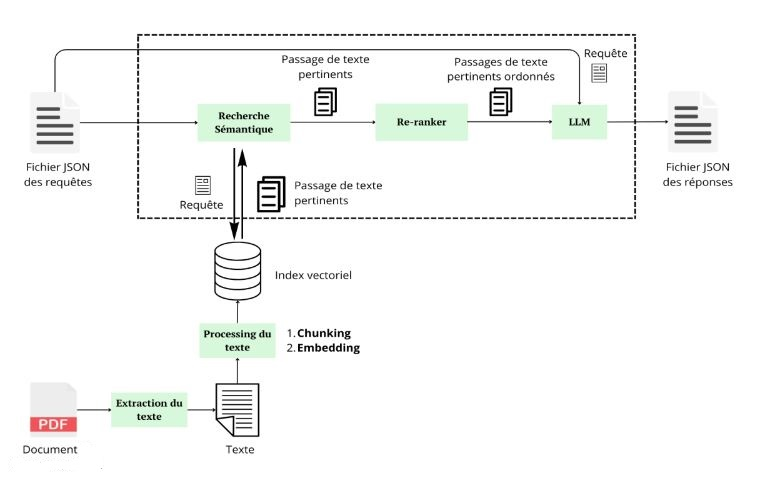
\includegraphics[scale=0.8]{rag.jpg}
    \caption{RAG system}
    \label{fig:mesh1}
\end{figure}
\newpage

\subsection{Benchmark}
Grâce à l'apport considérable du département DFS, nous avons pu établir un benchmark représentant un répertoire de 90 questions typiques aux fonds, une collecte de feuilles excel a été effectué, nous avons pu tester et évaluer les modèles, l'influence des changements d'architecture/modèles (embeddings,reranking), l'optimisation de l'utilisation mémoire en détérminant le nombre optimal de segments de texte à récupérer.


\subsection{Résultats}

Une fois le système mis en place avec des composants retournant des résultats acceptables, nous avons benchmarké les modèles open-source à notre disposition grâce à notre architecture définie précédemment. Le plus performant a été Mistral Instruct-v0.2 7B, qui malgré sa taille relativement petite comparée aux autres modèles utilisés dans l'industrie, a pu démontrer des résultats très corrects, illustrés dans l'histogramme ci-dessous :

\begin{figure}[h]
    \centering
\begin{tikzpicture}
\begin{axis}[
    ybar stacked,
    symbolic x coords={P1, P2,  P3, P4,  P5, P6,  P7, P8},
    xtick=data,
    ymin=0, ymax=90,
    bar width=20pt,
    ylabel={Nombre de réponses},
    xlabel={Prospectus},
    enlarge x limits=0.15,
    ymajorgrids=true,
    grid style=dashed,
    width=12cm,
    height=8cm,
    legend style={at={(0.5,-0.15)},
        anchor=north,legend columns=-1},
    area legend
]

\addplot+[
    ybar,
    draw=black,
    fill=green
] plot coordinates {
    (P1, 88)
    (P2, 84)
    (P3, 83)
    (P4, 84)
    (P5, 80)
    (P6, 80)
    (P7, 88)
    (P8, 82)
};

\addplot+[
    ybar,
    draw=black,
    fill=orange
] plot coordinates {
    (P1, 0)
    (P2, 1)
    (P3, 6)
    (P4, 3)
    (P5, 3)
    (P6, 8)
    (P7, 1)
    (P8, 6)
};

\addplot+[
    ybar,
    draw=black,
    fill=red
] plot coordinates {
    (P1, 2)
    (P2, 5)
    (P3, 1)
    (P4, 3)
    (P5, 7)
    (P6, 2)
    (P7, 1)
    (P8, 2)
};

\legend{Correct + Source, Discutable, Erreurs}

\end{axis}
\end{tikzpicture}
    \caption{Performance du RAG sur les prospectus}
    \label{fig:mesh2}
\end{figure}

Nous avons également effectué des tests avec des modèles propriétaires tels que GPT-3.5 Turbo et GPT-4 via AzureML (APIGEE). Bien que ces modèles aient montré des performances globalement supérieures, proches de 100\%, une comparaison relative taille/performance met Mistral en avant, surtout en raison de sa petite taille et de son efficacité. Cependant, il est important de noter que l'hébergement de modèles open-source présente des défis d'infrastructure et de maintenance par rapport à l'utilisation d'APIs, qui bien que simples à mettre en production, peuvent introduire des limitations et des coûts supplémentaires non négligeables.

\subsection{Perspectives:}
Le code ainsi que les résultats a été transmis à l'équipe concernée par le passage en production ausein de BP2S, l'évaluation et reporting ont été effectués en début d'été.
\newpage

\section{ \Large \bf Troisième Mission : Contribution d'un PDF Parser à une bibliothèque interne RAG-toolbox}

\subsection{Contexte et Objectif}

Dans le cadre de mon alternance chez BNP Paribas, j'ai été amené à travailler sur un projet de grande envergure visant à automatiser l'extraction d'informations complexes depuis des documents PDF. Cette mission, qui a débuté en mai 2024, s'inscrit dans une initiative plus large menée par le département BNP Pace, visant à développer une bibliothèque nommée \texttt{rag\_toolbox}. Cette bibliothèque a pour but de remplacer les utilitaires couramment utilisés autour de l'architecture RAG (Retrieval-Augmented Generation) par une solution interne, robuste et adaptable à divers formats de documents, incluant HTML, Markdown, DOCX, et surtout PDF.

L'objectif spécifique de ma mission était de concevoir et d'implémenter une solution capable d'extraire de manière cohérente et hiérarchique les informations contenues dans des PDF, tout en respectant les structures et les éléments visuels tels que les sections, les tableaux, les images, et autres éléments graphiques.

\textit{Référence à l'appendix : Une discussion sur les défis de l'extraction d'information à partir de PDF, et les techniques utilisées, est disponible dans \textbf{Appendix E}.}

\subsection{Méthodologie et Développement}

\subsubsection{\normalsize{Version Vanille avec PyMuPDF}}

La première étape de cette mission consistait à développer une version initiale de l'extracteur de PDF en utilisant la bibliothèque PyMuPDF. Cette version "vanille" se base sur l'analyse structurelle du document en exploitant les propriétés intrinsèques du texte, telles que la taille de la police, le style (gras, italique), et les correspondances regex pour les numérotations de sections (par exemple, \texttt{1.1.1}, \texttt{IV.1.a}, etc.).

L'extracteur a été conçu pour diviser le document en sections cohérentes, en suivant la hiérarchie implicite définie par les auteurs du document. Cette segmentation est essentielle pour permettre un traitement ultérieur précis et pour faciliter l'intégration de ces données dans des pipelines de traitement du langage naturel (NLP).


\subsubsection{\normalsize Implémentation et Qualité du Code}

Pour garantir la robustesse et la maintenabilité du code, des pratiques rigoureuses ont été mises en place, incluant l'utilisation de \texttt{pydantic} pour la validation des données, \texttt{mypy} pour le typage statique, et \texttt{pytest} pour les tests unitaires et d'intégration. Ces pratiques sont d'autant plus cruciales dans un contexte de pipeline d'intégration continue (CI), où le code doit passer des vérifications automatiques avant d'être déployé en production.


\subsubsection{\normalsize Intégration de YOLOv10 pour l'Extraction Avancée}

La deuxième phase du projet, encore en cours, vise à intégrer YOLOv10 (You Only Look Once) pour l'extraction d'éléments complexes tels que les tableaux, diagrammes, figures, et images dans les documents PDF. YOLOv10, qui inclut désormais des mécanismes d'attention, a été fine-tuné sur le dataset DocLayNet, ce qui a permis d'introduire de nouveaux labels spécifiquement adaptés aux documents structurés.

\textit{Référence à l'appendix : Les principes de base des modèles de vision comme YOLO, ainsi que leur adaptation aux documents structurés, sont détaillés dans \textbf{Appendix E}.}

L'intégration de YOLOv10 dans \texttt{rag\_toolbox} permet aux utilisateurs de choisir entre différentes méthodes d'extraction, en fonction de la complexité du document et des besoins spécifiques. Le transfert d'apprentissage (\textit{transfer learning}) est également envisagé pour adapter YOLOv10 à des cas d'usage spécifiques de BNP Paribas, tels que la détection de diagrammes, de figures, ou d'images non significatives.

\textit{Référence à l'appendix : Les concepts de \textit{transfer learning} et leur application dans le cadre des modèles de vision sont expliqués en profondeur dans \textbf{Appendix E}.}

\subsection{Résultats et Impact}

La version initiale de l'extracteur a montré une robustesse satisfaisante dans la segmentation des documents PDF, facilitant l'automatisation des processus de conformité et d'analyse réglementaire. L'intégration de YOLOv10 devrait encore améliorer la précision et l'efficacité de l'extraction des informations, en particulier pour les documents contenant des éléments graphiques complexes.

Cette mission a permis de renforcer l'autonomie de BNP Paribas dans le traitement de documents complexes, réduisant ainsi la dépendance à des solutions externes comme LangChain, Unstructured..etc, tout en offrant des fonctionnalités adaptées aux besoins spécifiques de l'entreprise.

\section{ Contributions diverses au travail des collègues:}
Ce point est très important pour moi, étant dans une équipe diversifiée et traitant plusieurs sujets, j'ai pu contribuer à une variété de problématiques, en commençant par des problèmes similaires aux miens rencontré par les stagiaires passés par l'équipe d'Emmanuel Chauvin, ensuite ceci se développa à plusieurs contributions lors de ma transition vers l'Innovation Lab, allant des isolations forests et réseaux de neurones profonds appliqués aux séries temporelles dans un contexte de détection de fraude jusqu'aux knowledge graphs dans un contexte de vérification de conformité réglementaire. Ceci constitue un pilier important de la réussite de mon alternance, car cela me permet de me former sur des sujets variés et toucher aux différentes tendances de l'industrie.


\section{Perspectives}
Les prochaines étapes consistent à finaliser l'intégration de YOLOv10 et à approfondir l'exploration de l'apprentissage par transfert pour affiner et adapter les modèles de détection aux labels spécifiques à nos documents. Par ailleurs, une attention particulière sera portée à la maintenance du code et élargir notre scope de contributions, afin d'assurer la robustesse et fiabilité de la bibliothèque.

En ce qui concerne mes perspectives futures, je suis actuellement en quête d'un sujet plus théorique au sein de l'Innovation Lab, avec l'ambition de potentiellement engager une démarche CIFRE pour poursuivre mes recherches dans un cadre académique tout en restant en lien avec les besoins industriels.






\newpage
\section{ \Large \bf Appendix:}
\appendix
\section{Fondements Mathématiques des Modèles de Langage}

\subsection{Probabilités Appliquées aux Modèles de Langage}

Les modèles de langage se fondent sur des principes de probabilités, permettant de quantifier la plausibilité de séquences de mots données dans un corpus. Considérons un vocabulaire $\mathcal{V}$ contenant l'ensemble des mots possibles. Soit $w_1, w_2, \dots, w_T$ une séquence de mots de longueur $T$. Un modèle de langage est défini par la probabilité jointe de cette séquence, notée $P(w_1, w_2, \dots, w_T)$, qui peut être décomposée selon la règle de la chaîne en un produit de probabilités conditionnelles :
\[
P(w_1, w_2, \dots, w_T) = P(w_1) \prod_{t=2}^{T} P(w_t | w_1, w_2, \dots, w_{t-1})
\]
Cette décomposition permet d'évaluer la probabilité de chaque mot de la séquence en fonction des mots qui le précèdent. 

Pour formuler de manière rigoureuse les modèles de langage dans le cadre de la théorie des probabilités, nous faisons appel à la théorie de la mesure. Soit $(\Omega, \mathcal{F}, P)$ un espace de probabilité où $\Omega$ est un ensemble des possibles, $\mathcal{F}$ une $\sigma$-algèbre sur $\Omega$, et $P$ une mesure de probabilité. Les séquences de mots peuvent être vues comme des éléments de $\Omega$, et les probabilités jointes comme des mesures sur cet espace.

Dans cette optique, la probabilité conditionnelle $P(w_t | w_1, w_2, \dots, w_{t-1})$ peut être interprétée comme la probabilité d'un événement conditionné par un sous-ensemble de $\mathcal{F}$. Plus formellement, si $A, B \in \mathcal{F}$ avec $P(B) > 0$, la probabilité conditionnelle est définie comme :
\[
P(A|B) = \frac{P(A \cap B)}{P(B)}
\]
Ce concept est fondamental dans l'établissement des relations de dépendance entre les mots dans une séquence.

\subsubsection{Tightness d'un Modèle}
Le concept de \textit{tightness} est crucial pour évaluer la capacité d'un modèle probabiliste à capturer fidèlement la distribution réelle des données. Mathématiquement, il peut être évalué via la divergence de Kullback-Leibler (KL), qui mesure la différence entre deux distributions de probabilité :
\[
D_{KL}(P \| Q) = \sum_{w \in \mathcal{V}} P(w) \log \frac{P(w)}{Q(w)}
\]
où $P$ est la distribution réelle des données et $Q$ est la distribution prédite par le modèle. Un modèle est considéré comme \textit{tight} si $D_{KL}(P \| Q)$ est faible, ce qui signifie que la distribution prédite $Q$ est proche de la distribution réelle $P$. Cela est particulièrement important lors du fine-tuning d'un modèle, où l'objectif est de minimiser cette divergence pour améliorer la généralisation tout en évitant le sur-apprentissage.

Un modèle est dit \textit{tight} si la somme des probabilités sur toutes les séquences possibles (finies) est égale à 1 :
\[
\sum_{w \in \mathcal{V}^*} P(w) = 1
\]
Dans le cas contraire, le modèle est non-tight et une partie de la masse de probabilité est perdue.

\subsection{Modèles Traditionnels de Langage}

\subsubsection{Modèles n-grammes}
Les modèles n-grammes sont parmi les approches les plus anciennes pour la modélisation de langage. Ils sont basés sur l'idée que la probabilité d'un mot donné ne dépend que d'une fenêtre glissante des $n-1$ mots qui le précèdent, ce qui se formalise comme suit :
\[
P(w_t | w_1, w_2, \dots, w_{t-1}) \approx P(w_t | w_{t-n+1}, \dots, w_{t-1})
\]
Cependant, pour des valeurs de $n$ plus élevées, le nombre de paramètres nécessaires pour estimer ces probabilités augmente exponentiellement, ce qui mène à un problème de sparsité des données. 

Pour résoudre ce problème, les techniques de \textit{smoothing} telles que le lissage de Laplace sont utilisées. Ce lissage ajoute une petite constante $\alpha$ à chaque fréquence de n-grammes, pour éviter les zéros dans les estimations de probabilité :
\[
P(w_t | w_{t-n+1}, \dots, w_{t-1}) = \frac{\text{count}(w_{t-n+1}, \dots, w_{t-1}, w_t) + \alpha}{\text{count}(w_{t-n+1}, \dots, w_{t-1}) + \alpha |\mathcal{V}|}
\]

\subsubsection{Modèles Basés sur le Lexique et le Vocabulaire}
Les modèles lexicaux se concentrent sur l'exploitation des relations sémantiques entre les mots. Par exemple, les techniques d'embeddings de mots comme Word2Vec ou GloVe capturent ces relations en représentant chaque mot par un vecteur dans un espace de dimension réduite. 

L'objectif de ces modèles est de maximiser la similarité des vecteurs pour les mots apparaissant dans des contextes similaires :
\[
\max_{\mathbf{w}} \sum_{\text{contexte}(w)} \log P(\text{contexte}(w) | \mathbf{w})
\]
où $\mathbf{w}$ est le vecteur d'embedding du mot $w$.

\subsubsection{Réseaux de Neurones Récurrents (RNN)}
Les RNNs introduisent une dynamique séquentielle dans les modèles de langage en permettant une récurrence dans le traitement des séquences de texte. À chaque étape $t$, un état caché $h_t$ est mis à jour en fonction de l'entrée actuelle $x_t$ et de l'état caché précédent $h_{t-1}$ :
\[
h_t = \tanh(W_h h_{t-1} + W_x x_t + b_h)
\]
Les RNNs peuvent être interprétés mathématiquement comme des systèmes dynamiques discrets, où chaque état est une fonction des états précédents et des nouvelles entrées.

\subsubsection{Long Short-Term Memory (LSTM)}
Les LSTM étendent les RNNs en introduisant des mécanismes pour mieux gérer les dépendances à long terme dans les séquences. La dynamique des LSTM est régie par des équations impliquant des portes d'entrée, de sortie et d'oubli :
\[
\begin{aligned}
    f_t &= \sigma(W_f \cdot [h_{t-1}, x_t] + b_f) \\
    i_t &= \sigma(W_i \cdot [h_{t-1}, x_t] + b_i) \\
    o_t &= \sigma(W_o \cdot [h_{t-1}, x_t] + b_o) \\
    \tilde{C}_t &= \tanh(W_C \cdot [h_{t-1}, x_t] + b_C) \\
    C_t &= f_t \cdot C_{t-1} + i_t \cdot \tilde{C}_t \\
    h_t &= o_t \cdot \tanh(C_t)
\end{aligned}
\]
Les LSTM permettent de conserver des informations sur des périodes prolongées et d'atténuer les problèmes de gradients, en s'assurant que les gradients peuvent circuler à travers le réseau sans disparaître ni exploser.

\subsubsection{Autoencodeurs Variationnels (VAE)}
Les VAE sont des modèles génératifs qui codent les données dans un espace latent continu et les régénèrent par un décodeur. La fonction de coût des VAE est composée de deux termes : une entropie croisée pour la reconstruction et une divergence de Kullback-Leibler pour régulariser l'espace latent :
\[
\mathcal{L}(\theta, \phi) = \mathbb{E}_{q_\phi(z|x)}[\log p_\theta(x|z)] - D_{KL}(q_\phi(z|x) \| p(z))
\]
Les VAE sont particulièrement utiles pour la génération de séquences complexes où il est essentiel de capturer une diversité dans les échantillons générés.

\section{Transformers et Mécanismes d'Attention}

\subsection{Introduction aux Transformers}

Les Transformers, introduits par Vaswani et al. en 2017, ont établi une nouvelle norme dans le traitement séquentiel en utilisant un mécanisme d'attention auto-régressive, remplaçant les architectures récurrentes traditionnelles. Formulons cela de manière formelle.

\subsubsection{Formulation Mathématique des Transformers}

Soit $\mathcal{T}$ un Transformer défini comme un tuple $\mathcal{T} = (\Sigma, D, \text{enc}_{\mathcal{T}})$, où :
\begin{itemize}
    \item $\Sigma$ est l'alphabet des symboles d'entrée,
    \item $D$ est la dimension du modèle,
    \item $\text{enc}_{\mathcal{T}}$ est la fonction d'encodage du Transformer.
\end{itemize}

Le Transformer maintient des encodages contextuels pour chaque symbole dans une séquence, permettant un accès direct aux informations de tous les symboles précédents. Contrairement aux RNNs, où un seul état caché est mis à jour séquentiellement, le Transformer conserve explicitement les encodages de tous les symboles, résolvant ainsi le problème de compression de l'information.

\subsubsection{Attention Scaled Dot-Product}

Le mécanisme d'attention dans les Transformers est basé sur la similarité entre les vecteurs de requêtes ($Q$), de clés ($K$) et de valeurs ($V$). Formulons cela précisément. Soit $Q \in \mathbb{R}^{n \times d_k}$, $K \in \mathbb{R}^{m \times d_k}$, et $V \in \mathbb{R}^{m \times d_v}$ où $n$ est la longueur de la séquence de requêtes, $m$ est la longueur de la séquence de clés, $d_k$ et $d_v$ sont les dimensions respectives des clés et valeurs.

L'attention \textit{scaled dot-product} est définie par :
\[
\text{Attention}(Q, K, V) = \text{softmax}\left(\frac{QK^\top}{\sqrt{d_k}}\right)V
\]
où $\sqrt{d_k}$ est un facteur de normalisation nécessaire pour éviter que les produits scalaires $QK^\top$ ne croissent trop en dimension élevée, ce qui pourrait rendre la fonction softmax extrêmement pointue et causer des gradients instables.

\subsubsection{Attention Multi-Têtes}

Pour permettre au modèle de capturer différentes relations contextuelles, les Transformers utilisent une attention multi-têtes. Formellement, soit $h$ le nombre de têtes d'attention, chaque tête $i$ effectue une attention \textit{scaled dot-product} avec ses propres matrices de poids $W_i^Q \in \mathbb{R}^{d_{model} \times d_k}$, $W_i^K \in \mathbb{R}^{d_{model} \times d_k}$, et $W_i^V \in \mathbb{R}^{d_{model} \times d_v}$ :

\[
\text{head}_i = \text{Attention}(QW_i^Q, KW_i^K, VW_i^V)
\]

Les résultats des $h$ têtes sont ensuite concaténés et projetés par une couche linéaire $W^O \in \mathbb{R}^{hd_v \times d_{model}}$ :

\[
\text{MultiHead}(Q, K, V) = \text{Concat}(\text{head}_1, \dots, \text{head}_h)W^O
\]

\subsection{Propriétés de Scaling et Complexité}

Les Transformers se distinguent par leur capacité à traiter des séquences longues en parallèle. Définissons formellement la complexité. Soit $n$ la longueur de la séquence, la complexité en temps et en espace de l'attention est quadratique, c'est-à-dire $O(n^2)$. Cette complexité provient de la nécessité de calculer les produits scalaires entre toutes les paires d'éléments dans la séquence :

\[
\text{Complexité en temps/espaces} = O(n^2)
\]

Pour réduire cette complexité, diverses approches ont été proposées, comme l'attention approximative qui calcule les produits scalaires de manière éparse ou sur une sous-sélection d'éléments de la séquence, réduisant ainsi la charge computationnelle au prix d'une perte potentielle de précision.

\subsection{Problématiques Associées aux Transformers}

\subsubsection{Boîte Noire et Problèmes d'Explicabilité}

Les Transformers, malgré leurs performances inégalées, présentent des défis en termes d'explicabilité. Formellement, cela signifie que la fonction de décision $\mathcal{D}(x)$, où $x$ est une entrée, est complexe à interpréter, ce qui rend difficile l'explication des décisions prises par le modèle, notamment dans des domaines critiques.

\subsubsection{Complexité Computationnelle}

La complexité quadratique des Transformers les rend impraticables pour des séquences extrêmement longues ou dans des environnements à ressources limitées. Des variantes telles que les Linformers et les Réformers ont été proposées pour améliorer l'efficacité, mais elles impliquent des compromis. Par exemple, le modèle Linformer réduit la complexité à $O(n)$ en projetant les clés et valeurs dans un espace de dimension fixe, mais au coût d'une perte potentielle d'information contextuelle.

\section{Fine-Tuning des Modèles de Langage}

\subsection{Supervised Fine-Tuning (SFT)}

Le \textit{fine-tuning} supervisé ajuste les poids $\theta$ d'un modèle pré-entraîné sur un nouveau jeu de données $\mathcal{D} = \{(x_i, y_i)\}_{i=1}^N$. Le processus consiste à minimiser la fonction de perte, typiquement l'entropie croisée, définie par :

\[
\mathcal{L}(\theta) = -\frac{1}{N} \sum_{i=1}^{N} y_i \log P(y_i | x_i; \theta)
\]

où $P(y_i | x_i; \theta)$ représente la probabilité prédite pour l'étiquette $y_i$ donnée l'entrée $x_i$ et les paramètres $\theta$.

\subsection{LoRA (Low-Rank Adaptation)}

LoRA (\textit{Low-Rank Adaptation}) est une technique qui permet de fine-tuner un grand modèle de langage sans avoir à modifier l'intégralité de ses poids. Au lieu de mettre à jour tous les paramètres du modèle, LoRA gèle les poids d'origine et introduit de petites matrices appelées \textit{adapters}, qui sont entraînées pour capturer les informations nécessaires à l'adaptation du modèle.

Formellement, considérons les poids d'une couche $W \in \mathbb{R}^{d_{out} \times d_{in}}$. Dans LoRA, les poids d'origine $W$ sont conservés, et une mise à jour $\Delta W$ est appliquée sous la forme d'une décomposition en deux matrices de faible rang $A \in \mathbb{R}^{d_{out} \times r}$ et $B \in \mathbb{R}^{r \times d_{in}}$, où $r \ll \min(d_{out}, d_{in})$. Cette mise à jour se formalise ainsi :

\[
W' = W + A \times B
\]

Les matrices $A$ et $B$ sont les seules à être entraînées, ce qui permet de réduire significativement le nombre total de paramètres à ajuster, rendant le \textit{fine-tuning} plus efficace et moins coûteux en ressources. Cette approche est particulièrement utile pour adapter des modèles de très grande taille à des tâches spécifiques, tout en minimisant l'empreinte mémoire et les besoins en calculs [\cite{Hu2021}].


\subsection{Quantification et QLoRA}

La quantification est une méthode visant à optimiser les modèles de langage en réduisant la précision numérique des poids des réseaux de neurones, ce qui diminue leur taille et les exigences computationnelles. Considérons un poids $W \in \mathbb{R}^d$, où $d$ est la dimension du poids dans l'espace flottant à haute précision (par exemple, FP32). Le processus de quantification transforme ce poids en un poids quantifié $W_q \in \mathbb{Q}^k$, où $k$ est la précision réduite (par exemple, INT8), selon la relation suivante :

\[
W_q = \text{round}\left(\frac{W - z}{\text{scale}}\right) + z_q
\]

où $\text{scale}$ est un facteur de mise à l'échelle calculé pour minimiser la perte de précision, $z$ est un offset de quantification pour aligner les plages de valeurs, et $z_q$ est l'offset quantifié. La fonction \text{round} arrondit le résultat à l'entier le plus proche, convertissant ainsi les poids en une représentation à plus faible précision.

Plusieurs méthodes avancées de quantification existent :
\begin{itemize}
    \item \textbf{GPTQ} : Cette méthode convertit les poids en entiers de faible précision (INT4 ou INT8) tout en maintenant les gradients pendant la rétropropagation grâce à une factorisation de Cholesky. GPTQ optimise les poids de chaque couche pour minimiser l'erreur introduite par la quantification, permettant ainsi de préserver les performances du modèle tout en réduisant considérablement l'empreinte mémoire.
     \item \textbf{NF4 (NormalFloat 4-bit)} : NF4 est une méthode qui utilise une quantification en 4 bits basée sur des quantiles, permettant un ajustement flexible entre précision et mémoire. Couplée avec la Double Quantization, elle permet de réduire la consommation mémoire tout en conservant une bonne précision, particulièrement utile dans des scénarios de \textit{fine-tuning} avec des techniques comme QLoRA.
    \item \textbf{GGUF (General Quantized Uniform Format)} : GGUF est une méthode récente qui améliore la quantification en uniformisant la représentation des poids sur plusieurs couches du réseau de neurones. Elle applique une quantification uniforme à tous les poids d'un modèle, ce qui simplifie l'implémentation tout en assurant une dégradation minimale des performances. GGUF est particulièrement avantageux pour les modèles nécessitant une compatibilité entre différentes architectures matérielles, en garantissant une efficacité élevée même sur des systèmes hétérogènes.
\end{itemize}

\textbf{QLoRA} tire parti de ces méthodes de quantification pour permettre un \textit{fine-tuning} efficace des grands modèles. En combinant la quantification (comme NF4 ou GGUF) avec LoRA, il est possible de n'ajuster qu'une petite partie des paramètres du modèle, ce qui permet d'adapter de grands modèles à des environnements à ressources limitées tout en maintenant une haute performance. Cette approche est cruciale pour le déploiement de modèles massifs sur des infrastructures GPU avec une capacité mémoire réduite, tout en minimisant l'impact sur la précision du modèle.

\section{Génération de Données Synthétiques}

La génération de données synthétiques est essentielle pour augmenter la quantité de données disponibles pour l'entraînement des modèles de langage. Formulons le processus de manière formelle.

Soit un document $\mathcal{D}$ structuré en sections $S = \{S_1, S_2, \dots, S_n\}$, chaque section $S_i$ est découpée en segments cohérents $\{s_1^i, s_2^i, \dots\}$. Un modèle de langage $\mathcal{M}$ est ensuite utilisé pour générer des paires de questions-réponses $(q, r)$ pour chaque segment $s_j^i$.

Le processus est formalisé par l'application d'une fonction $\mathcal{G}$ qui prend en entrée un segment $s_j^i$ et génère une paire $(q, r)$ telle que :

\[
(q, r) = \mathcal{G}(s_j^i)
\]

Cela permet de créer un jeu de données $\mathcal{D}' = \{(q, r)\}$ riche et diversifié, qui peut être utilisé pour améliorer les performances du modèle $\mathcal{M}$ sur des tâches spécifiques.


\section{YOLOv10: Innovations et Applications}

\subsection{Introduction à YOLOv10}

YOLOv10 représente la dernière évolution dans la série des modèles YOLO (You Only Look Once), qui sont réputés pour leur efficacité en détection d'objets en temps réel. Ce modèle conserve les principes fondamentaux de ses prédécesseurs tout en introduisant des améliorations substantielles dans l'architecture et les mécanismes de post-traitement. Le pipeline de détection d'objets de YOLOv10 se compose de deux éléments essentiels : l'inférence et le post-traitement.

Dans les versions précédentes de YOLO, l'étape de post-traitement impliquait l'utilisation de la Non-Maximum Suppression (NMS) pour éliminer les prédictions redondantes. Bien que NMS soit efficace pour réduire les doublons, il introduit une latence supplémentaire dans le pipeline, impactant ainsi la vitesse d'inférence. YOLOv10 innove en supprimant la dépendance à NMS grâce à des \textit{affectations doubles cohérentes}, une méthode qui permet un entraînement sans NMS tout en maintenant une performance élevée et une faible latence.

\subsection{Entraînement de YOLOv10 par Transfer Learning}

Le \textit{transfer learning} est une stratégie clé pour l'efficacité de YOLOv10, en particulier lorsque le modèle est appliqué à des tâches spécifiques ou à des ensembles de données restreints. Soit un modèle YOLOv10 pré-entraîné sur un ensemble de données générique $D_g$, tel que COCO, qui permet d'apprendre des caractéristiques visuelles globales. Ensuite, un \textit{fine-tuning} est effectué sur un ensemble de données spécifique $D_s$, tel que DocLayNet, qui est adapté pour la détection de structures complexes dans les documents.

Formellement, si $\theta_g$ représente les paramètres du modèle pré-entraîné, le \textit{fine-tuning} consiste à optimiser ces paramètres sur $D_s$ pour minimiser une fonction de perte $\mathcal{L}$ spécifique à la tâche :
\[
\theta_s = \arg\min_{\theta} \mathcal{L}(\theta; D_s)
\]
où $\theta_s$ représente les paramètres ajustés. Ce processus permet d'affiner les capacités du modèle pour des tâches spécifiques tout en capitalisant sur les connaissances générales acquises durant le pré-entraînement.

\subsection{Utilisation de YOLOv10 pour l'Extraction d'Informations dans les Documents}

YOLOv10 s'avère particulièrement performant pour l'extraction d'informations visuelles à partir de documents complexes, tels que les PDF. En \textit{fine-tuning} sur un ensemble de données comme DocLayNet, YOLOv10 peut détecter et segmenter des éléments tels que les tableaux, figures, et diagrammes avec une grande précision, facilitant ainsi l'automatisation des processus de traitement de documents.

Formellement, soit $I$ une image représentant une page de document, YOLOv10 prédit un ensemble de boîtes englobantes $\{b_1, b_2, \dots, b_n\}$ avec leurs catégories respectives $\{c_1, c_2, \dots, c_n\}$. Ces prédictions sont ensuite utilisées pour extraire les informations pertinentes, améliorant ainsi l'efficacité du traitement de documents en temps réel.

\subsection{Innovations dans YOLOv10: Partial Attention et Suppression du NMS}

YOLOv10 introduit des innovations architecturales majeures, parmi lesquelles le mécanisme de \textit{partial attention}, qui permet au modèle de se concentrer sur les régions les plus pertinentes d'une image. Soit $x$ une image d'entrée, le mécanisme de \textit{partial attention} applique une fonction de pondération sur les pixels $x_i$ de l'image, déterminée par une matrice d'attention $A$ :
\[
\tilde{x}_i = A(x) \cdot x_i
\]
où $\tilde{x}_i$ représente les pixels pondérés. Cette méthode améliore la précision de la détection tout en réduisant le bruit.

Une autre avancée critique de YOLOv10 est l'élimination du besoin de NMS. En utilisant des \textit{affectations doubles cohérentes}, YOLOv10 génère des prédictions sans redondance directement à partir du modèle, ce qui supprime l'étape de NMS. Soit $P(y|x)$ la probabilité de prédiction pour une classe $y$ donnée une entrée $x$, le modèle ajuste cette probabilité en optimisant une fonction de perte de type softmax ajustée, qui intègre directement la non-redondance :
\[
P(y|x) = \frac{e^{\text{score}(y,x)}}{\sum_{y'} e^{\text{score}(y',x)}}
\]
Cette approche réduit la latence d'inférence et simplifie le pipeline de traitement.

\subsection{Avantages et Performances de YOLOv10}

YOLOv10 se distingue par une amélioration significative de l'efficacité par rapport à ses prédécesseurs. Comparé à YOLOv9-C, YOLOv10-B réduit la latence de 46 \% et le nombre de paramètres de 25 \%, tout en maintenant une précision comparable. Soit $T_{9}$ et $T_{10}$ les temps d'inférence respectifs de YOLOv9-C et YOLOv10-B :
\[
\frac{T_{10}}{T_{9}} \approx 0.54
\]
ce qui montre l'efficacité accrue de YOLOv10 et justifie son utilisation pour nos cas d'usages.

\vspace{2cm}
\hspace{1cm} 

\newpage




\begin{thebibliography}{5}


\bibitem{Hinton2015}
G. Hinton, O. Vinyals, and J. Dean, "Distilling the Knowledge in a Neural Network," arXiv preprint arXiv:1503.02531, 2015. [Online]. Available: https://arxiv.org/abs/1503.02531. 
\bibitem{Hu2021}
E. Hu, Y. Shen, P. Wallis, Z. Allen-Zhu, Y. Li, S. Wang, L. Wang, and W. Chen, "LoRA: Low-Rank Adaptation of Large Language Models," arXiv preprint arXiv:2106.09685, 2021. [Online]. Available: https://arxiv.org/abs/2106.09685.
\bibitem{YOLOv10_2024}
A. Wang, H. Chen, L. Liu, K. Chen, Z. Lin, J. Han, and G. Ding, "YOLOv10: Real-Time End-to-End Object Detection," arXiv preprint arXiv:2405.14458, 2024. [Online]. Available: https://arxiv.org/abs/2405.14458.
\bibitem{model}
https://github.com/moured/YOLOv10-Document-Layout-Analysis
\bibitem{Cotterell2024}
R. Cotterell, A. Svete, C. Meister, T. Liu, and L. Du, \textit{Formal Aspects of Language Modeling}, arXiv preprint arXiv:2311.04329, 2024. [Online]. Available: https://arxiv.org/abs/2311.04329.

\bibitem{RAG2020}
P. Lewis, E. Perez, A. Karpukhin, D. Yogatama, B. Stenetorp, and S. Riedel, "Retriever-Augmented Generation for Knowledge-Intensive NLP Tasks," in *Advances in Neural Information Processing Systems* (NeurIPS), 2020.
\bibitem{Transformer2017}
A. Vaswani, N. Shazeer, N. Parmar, et al., "Attention Is All You Need," in *Advances in Neural Information Processing Systems* (NeurIPS), 2017.



\end{thebibliography}





\end{document}
